\documentclass{article}

% Language setting
% Replace `English' with e.g. `Spanish' to change the document language
\usepackage[english]{babel}
\usepackage{longtable}

% Set page size and margins
% Replace `letter paper' with `a4paper' for UK/EU standard size d
\usepackage{hyperref}
\usepackage{setspace}
\setstretch{1.6}
\usepackage[letterpaper, margin=1in]{geometry}

% Useful packages
\usepackage{amsmath}
\usepackage{graphicx}
\usepackage[colorlinks=true, allcolors=blue]{hyperref}
\usepackage{adjustbox}
\usepackage{booktabs} % for better-looking tables
\usepackage{array} % for better column formatting
\usepackage[table]{xcolor} % for coloring tables
\usepackage{colortbl}
\usepackage[backend=biber,style=mla]{biblatex}
\addbibresource{references.bib} % The filename of your .bib file
\usepackage{booktabs} % For formal tables
\usepackage{siunitx} % Alignment for table numbers
\usepackage{graphicx} % Required for including images
\usepackage{float} % For table positioning


\title{\textbf{Which Groups Benefited Most from the 2006 Massachusetts Health Care Reform?}}
\author{\textbf{Team 12}}

\begin{document}


\begin{document}
\maketitle

\section*{}
We study the effects of the 2006 Massachusetts Health Care Reform on health insurance coverage rates. Using a difference-in-differences design, we find that the number of insured individuals decreased by five percentage points, or 60 percent. This decline is primarily driven by low-income and young individuals, whose uninsurance rate declines by 11 and 15 percentage points, respectively. This is consistent with these groups' lower baseline coverage rates and the reforms' expansion of programs to target these groups.

\newpage
\section*{Introduction/Literature Review}
The Massachusetts Health Care Reform was established in response to the 2005/6 Deficit Reduction Act passed during the Bush Administration. The Administration wanted to reduce the government budget deficit by sharing the costs of healthcare expenditures with individual states. This led to various state-level healthcare reforms across the country, one of which was Massachusetts. The Massachusetts reform made individuals and families with incomes up to 300\% of the Federal Poverty Level (FPL)  eligible for subsidies on their health insurance premiums. These subsidies were heterogeneous at 50\% intervals. For example, individuals with incomes under 150\% of the FPL had their health insurance completely subsidized,and then the subsidies decreased for each 50 percentage point increase in income over the FPL (and were 0 if income is over 300\% of the FPL.)

 The law established an individual mandate to purchase health insurance and fined individuals up to 50\% of the lowest cost premium they qualified for otherwise. It also required employers who have 11 or more employees to pay for their employees’ health insurance or face an annual fine of up to \$295 per employee. This act was a precursor to the 2010 Affordable Care Act, which attempted to scale the Massachusetts reform at the national level. Other states were also required to adjust their healthcare policies as a result of the Deficit Reduction Act, but no state (besides Vermont which passed their healthcare reform in 2007) was able to achieve close to universal coverage.


Previous literature has discussed the effects of the Massachusetts Health Care reform on healthcare outcomes. This literature has found improved general health outcomes such as Emergency Room admission (Miller 2012,  Van der Rees et al 2013), reduced financial difficulties through higher credit scores and reduced likelihood of personal bankruptcy Mazumder and Miller (2016), and increased healthcare access (Miller 2012, Pande et al 2011). Mazumder and Miller (2016) use a triple differences design to control for differential trends in age.

\section*{Data description}
We supplemented the cpsinsure.dta dataset provided with CPS core data. We do this by adding more detailed data on demographics, insurance outcomes, labour statistics, and education characteristics. 

\section*{Empirical Strategy}
\subsection*{Difference in Differences}
Our goal is to estimate the average treatment effect of the treated (ATET) units for health insurance takeup and age. We do this by using a simple difference in differences design where our outcome is $Y_{sti}$, a dummy variable representing whether individual $i$ in state $s$ at year $t$ has health insurance coverage. We define $\alpha_s$ to be a state fixed effect, $\delta_t$ to be a year fixed effect, and $\delta$ to be an individual fixed-effect. $Reform_s$ is defined as a binary treatment variable taking value 1 if the state is Massachusetts and taking value 0 if not. The indicator variable simply indicates whether $\tau$ is equal to $t$. We run the regression separately for low-income and young individuals when examining heterogeneous treatment effects.

\begin{equation}
Y_{i s t}=\alpha_i+\alpha_s+\delta_t+\sum_{\substack{\tau=2001 \tau,  \neq 2006}}^{2013} \beta_\tau\left(\operatorname{Reform}_s \times I(t=\tau)\right)+\epsilon_{i s t}
\end{equation}

We use New Hampshire, Connecticut, Rhode Island, and Maine as our control group. (ie $Reform_s = 0$). We exclude Vermont because it enacted a similar reform to Massachusetts in 2007, which would lead to a negatively biased estimate of health insurance uptake. This represents most states in New England which we expect have similar demographic characteristics to Massachusetts as they are all predominantly white and highly educated relative to the rest of the country. In the below discussion, the outcome variable is the take up of health insurance.

For differences in differences to identifying ATET, we rely on the parallel trends assumption holding between our treated unit and control units in each of our specifications. The parallel trends assumption requires that in the absence of treatment, the trend in the take-up rates of insurance in Massachusetts must be the same as the trend in the take-up rates of insurance in the control group. To examine this, we test pretrends and demonstrate that pretrends are insignificant for each specification. This is shown in Figures 1-4. However, our identifying assumption could be violated if there are time shocks that affect control states more than Massachusetts. An example would be that perhaps the Great Recession in 2008 affected some states more than others. We show that our result is robust to excluding certain states that experienced a larger shock, such as Maine, mitigating this concern. 

Further we require the Stable Unit Treatment Value Assumption (SUTVA) to hold in our sample to insure that treatment effects in Massachusetts are not being biased by any extraneous factors. SUTVA is not violated insurance take up would not be plausibly affected by policy changes in other states. In extension, we need the treatment dummy to be uncorrelated with other unobservables, since this was a federally mandated policy change this is also likely to be satisfied.


We demonstrate through an event study that there was approximately a 0.05 reduction in the proportion of individuals uninsured in Figure 1. In figure 2 we show an approximately 0.05 increase in the proportion of individuals covered by insurance in Massachusetts. In figure 3, we show an approximately 0.11 reduction in the number of uninsured for individuals in the bottom income tercile and no reduction for those in the top income tercile. In figure 4 we show the heterogeneity of healthcare coverage by age. For young individuals, between ages 18-30 inclusive, we observe a 0.12 reduction in the proportion of individuals who are uninsured. This is statistically significant. For old individuals, between ages 50-64 inclusive, we observe a more muted 0.04 reduction in the proportion of individuals who are uninsured, which is initially insignificant, but becomes significant in 2012. The above results demonstrate that the 2006 Massachusetts Health Care Reform led to greater number of people insured, particularly those who are young and poor. 

This paper demonstrates that the reform accomplished at least some of what it was intending to do. There was an expansion of health care coverage to those who needed it, the poor, through the enrollment of more low risk young individuals. Consequently the Massachusetts Health Care Reform did what it was intended to- provide nearly universal health coverage. This was unique to the Massachusetts policy and other states which did not implement this policy did not achieve such stellar results. 
\newpage
\section*{Appendix}
Plots labeled (1-4) in ascending order. Coefficients are regression coefficients from the specification in the main text.
\begin{figure}
    \centering
    
\includegraphics[width=0.75\linewidth]{2.png}
\end{figure}

\begin{figure}
    \centering
    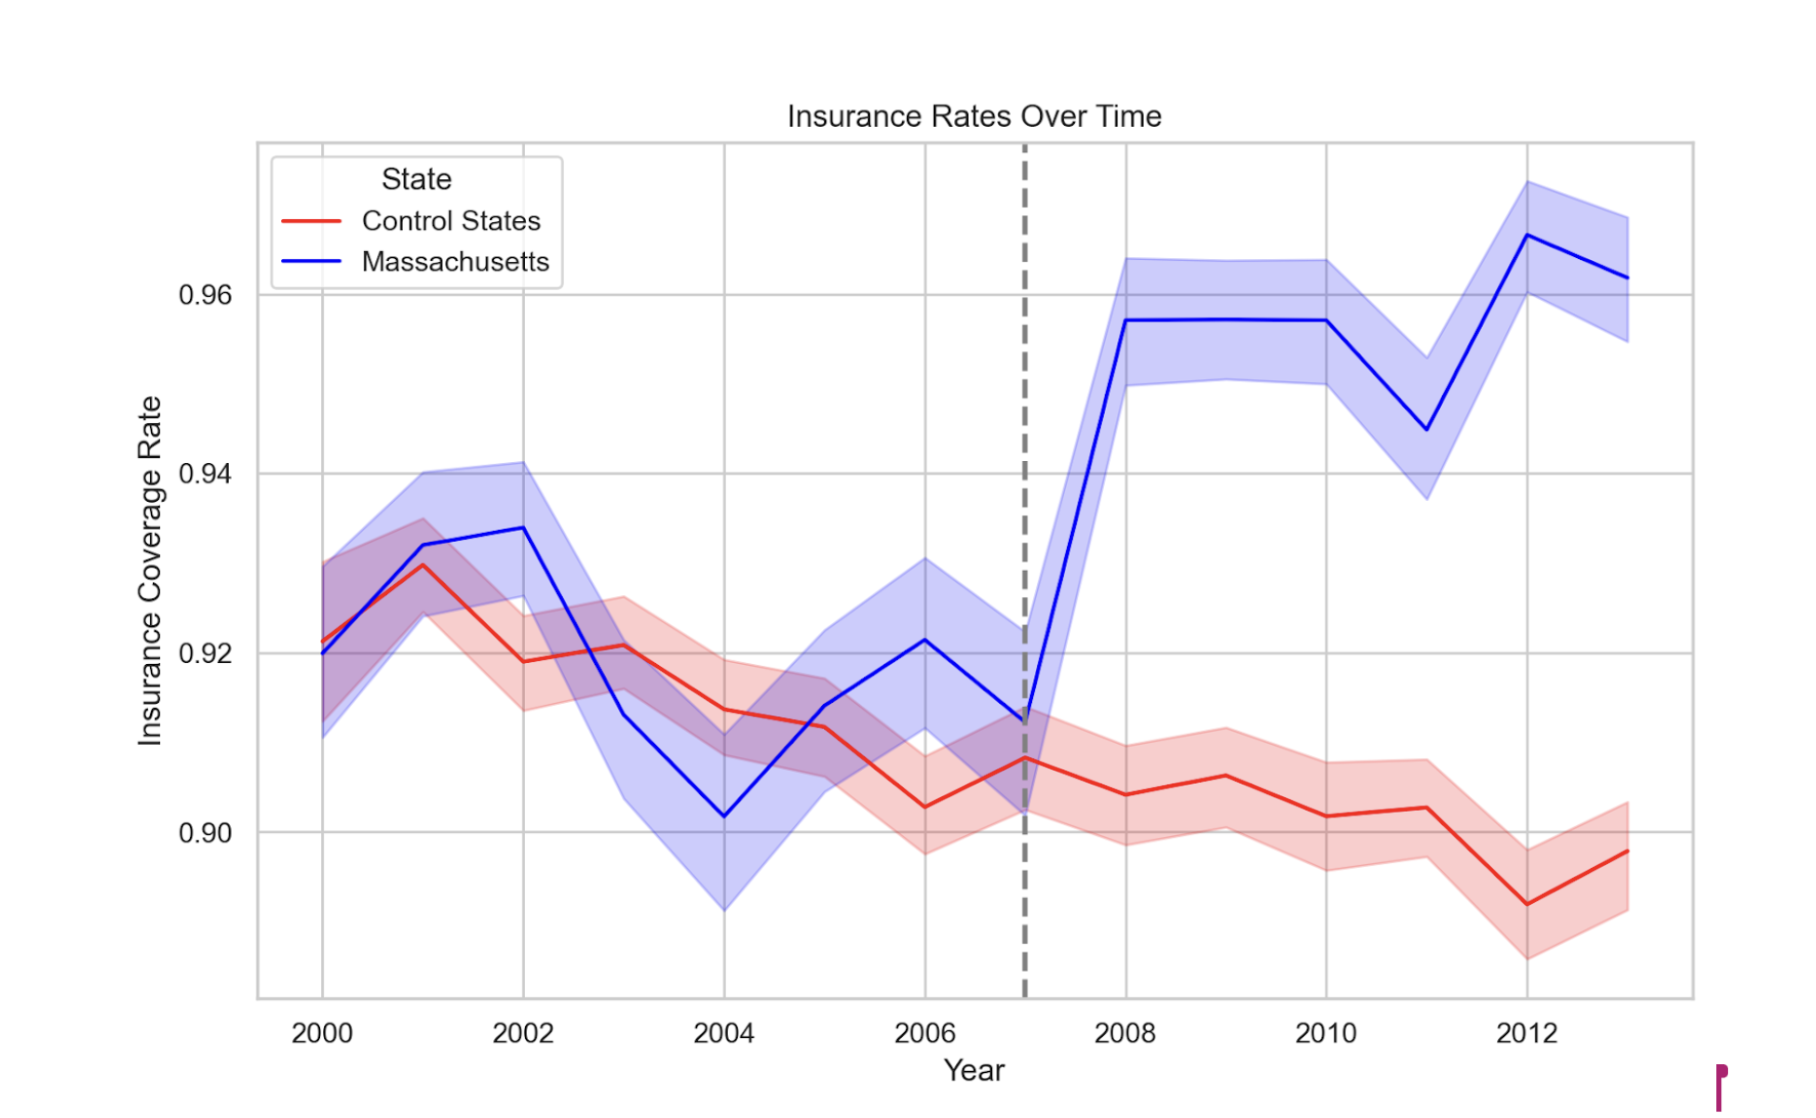
\includegraphics[width=0.75\linewidth]{3.png}
\end{figure}

\begin{figure}
\begin{figure}
        \centering
        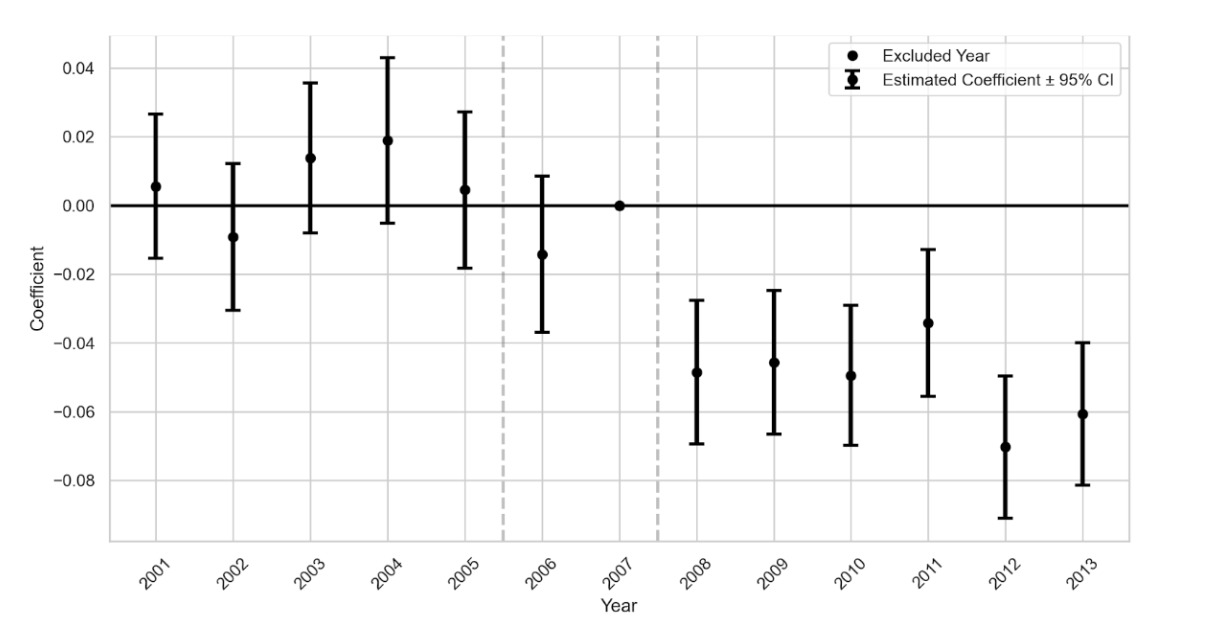
\includegraphics[width=0.75\linewidth]{5.png}
        \caption{Enter Caption}
        \label{fig:enter-label}
    \end{figure}
    \centering
    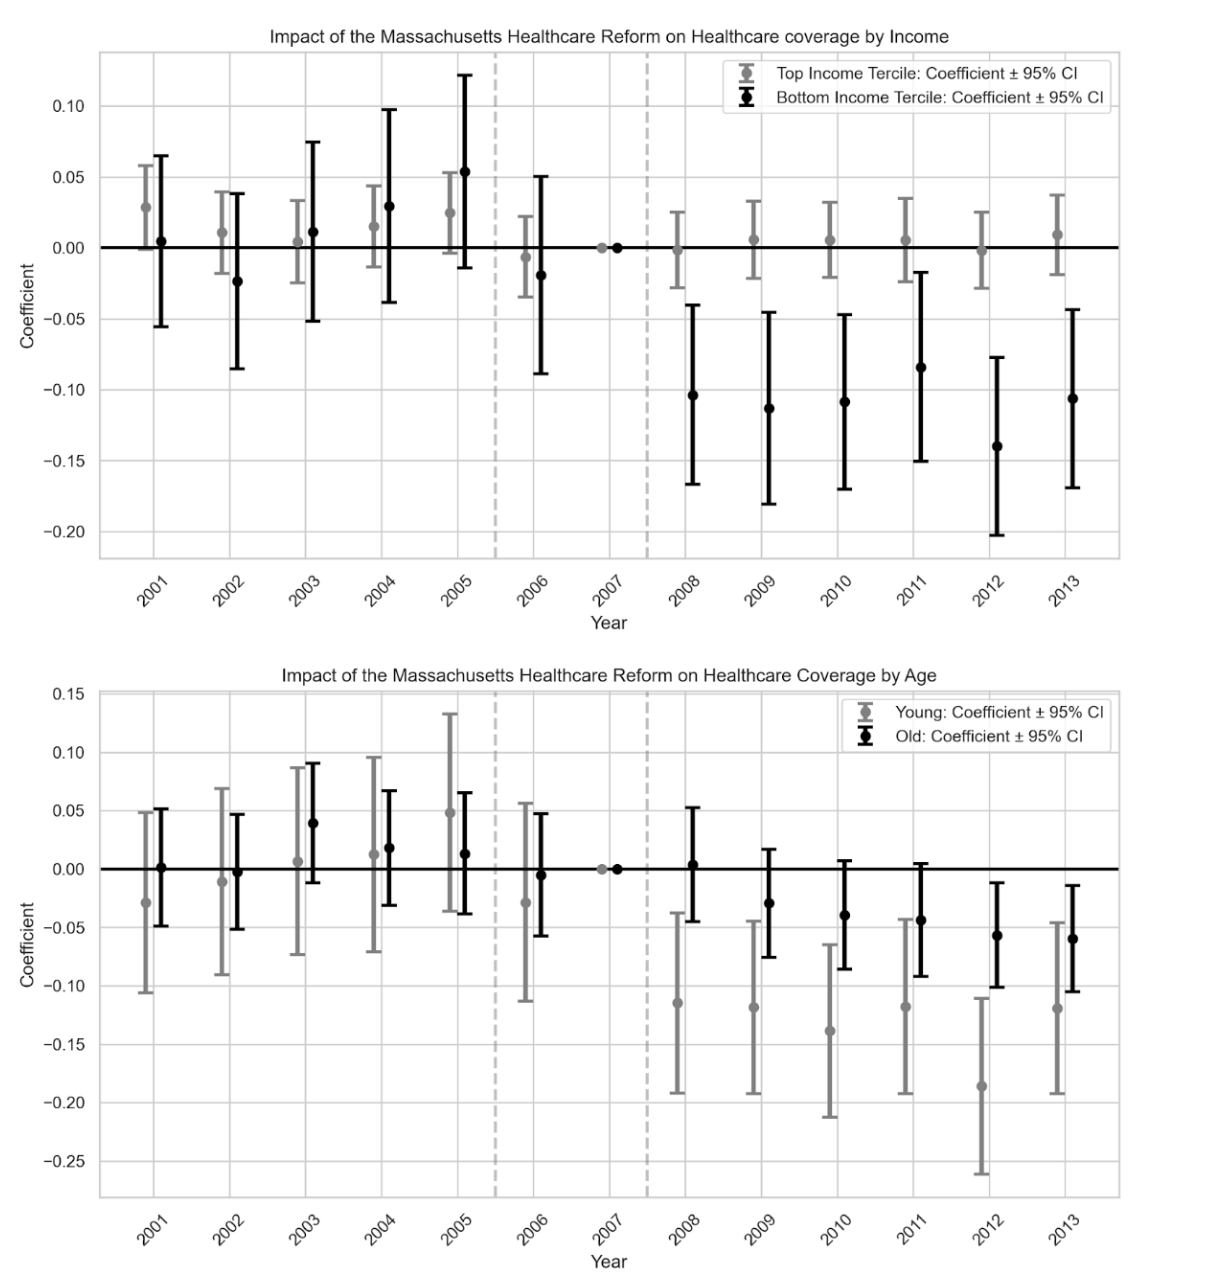
\includegraphics[width=0.75\linewidth]{4.png}
\end{figure}

\section*{References}
\newpage
\newpage
Milyo, Jeffrey, and Joel Waldfogel. 1999. "The Effect of Price Advertising on Prices: Evidence in the Wake of 44 Liquormart." American Economic Review, 89 (5): 1081-1096.

"Medicaid Long-Term Services Reforms in the Deficit Reduction Act." 2013. https://www.kff.org/wp-content/uploads/2013/01/7486.pdf. Accessed: 2016-04.

Kolstad, Jonathan T., and Amanda E. Kowalski. 2016. "Mandate-based health reform and the labor market: Evidence from the Massachusetts reform." Journal of Health Economics, pp. 1–26.

https://www.sciencedirect.com/science/article/abs/pii/S0167629616000278. DOI: 10.1016/j.jhealeco.2016.01.012.

Mazumder, Bhashkar, and Sarah Miller. 2016. "The Effects of the Massachusetts Health Reform on Household Financial Distress." American Economic Journal: Economic Policy, pp. 1–19.

https://pubs.aeaweb.org/doi/pdfplus/10.1257/pol.20150045. DOI: 10.1257/pol.20150045.

"2007 HHS Poverty Guidelines." 2007. https://aspe.hhs.gov/2007-hhs-poverty-guidelines.

"History of Health Reform." 2011. https://www.kff.org/wp-content/uploads/2011/03/5-02-13-history-of-health-reform.pdf.



\end{document}

